\ifx\wholebook\relax \else
% ------------------------ 

\documentclass{article}
%------------------- Other types of document example ------------------------
%
%\documentclass[twocolumn]{IEEEtran-new}
%\documentclass[12pt,twoside,draft]{IEEEtran}
%\documentstyle[9pt,twocolumn,technote,twoside]{IEEEtran}
%
%-----------------------------------------------------------------------------
%%
% loading packages
%
\newif\ifpdf
\ifx\pdfoutput\undefined % We're not running pdftex
  \pdffalse
\else
  \pdftrue
\fi
%
%
\ifpdf
  \RequirePackage[pdftex,%
            CJKbookmarks,%
       bookmarksnumbered,%
              colorlinks,%
          linkcolor=blue,%
              hyperindex,%
        plainpages=false,%
       pdfstartview=FitH]{hyperref}
\else
  \RequirePackage[dvipdfm,%
             CJKbookmarks,%
        bookmarksnumbered,%
               colorlinks,%
           linkcolor=blue,%
               hyperindex,%
         plainpages=false,%
        pdfstartview=FitH]{hyperref}
  \AtBeginDvi{\special{pdf:tounicode GBK-EUC-UCS2}} % GBK -> Unicode
\fi
\usepackage{hyperref}

% other packages
%-----------------------------------------------------------------------------
\usepackage{graphicx, color}
\usepackage{CJK}
%
% for programming 
%
\usepackage{verbatim}
\usepackage{listings}


\lstdefinelanguage{Smalltalk}{
  morekeywords={self,super,true,false,nil,thisContext}, % This is overkill
  morestring=[d]',
  morecomment=[s]{"}{"},
  alsoletter={\#:},
  escapechar={!},
  literate=
    {BANG}{!}1
    {UNDERSCORE}{\_}1
    {\\st}{Smalltalk}9 % convenience -- in case \st occurs in code
    % {'}{{\textquotesingle}}1 % replaced by upquote=true in \lstset
    {_}{{$\leftarrow$}}1
    {>>>}{{\sep}}1
    {^}{{$\uparrow$}}1
    {~}{{$\sim$}}1
    {-}{{\sf -\hspace{-0.13em}-}}1  % the goal is to make - the same width as +
    %{+}{\raisebox{0.08ex}{+}}1		% and to raise + off the baseline to match -
    {-->}{{\quad$\longrightarrow$\quad}}3
	, % Don't forget the comma at the end!
  tabsize=2
}[keywords,comments,strings]

\lstloadlanguages{C++, Lisp, Smalltalk}

% ======================================================================

\def\BibTeX{{\rm B\kern-.05em{\sc i\kern-.025em b}\kern-.08em
    T\kern-.1667em\lower.7ex\hbox{E}\kern-.125emX}}

\newtheorem{theorem}{Theorem}

%
% mathematics
%
\newcommand{\be}{\begin{equation}}
\newcommand{\ee}{\end{equation}}
\newcommand{\bmat}[1]{\left( \begin{array}{#1} }
\newcommand{\emat}{\end{array} \right) }
\newcommand{\VEC}[1]{\mbox{\boldmath $#1$}}

% numbered equation array
\newcommand{\bea}{\begin{eqnarray}}
\newcommand{\eea}{\end{eqnarray}}

% equation array not numbered
\newcommand{\bean}{\begin{eqnarray*}}
\newcommand{\eean}{\end{eqnarray*}}

\RequirePackage{CJK,CJKnumb,CJKulem,CJKpunct}
% we use CJK as default environment
\AtBeginDocument{\begin{CJK*}{GBK}{song}\CJKtilde\CJKindent\CJKcaption{GB}}
\AtEndDocument{\clearpage\end{CJK*}}

%
% loading packages
%
\newif\ifpdf
\ifx\pdfoutput\undefined % We're not running pdftex
  \pdffalse
\else
  \pdftrue
\fi
%
%
\ifpdf
  \RequirePackage[pdftex,%
       bookmarksnumbered,%
              colorlinks,%
          linkcolor=blue,%
              hyperindex,%
        plainpages=false,%
       pdfstartview=FitH]{hyperref}
\else
  \RequirePackage[dvipdfm,%
        bookmarksnumbered,%
               colorlinks,%
           linkcolor=blue,%
               hyperindex,%
         plainpages=false,%
        pdfstartview=FitH]{hyperref}
\fi
\usepackage{hyperref}

% other packages
%-----------------------------------------------------------------------------
\usepackage{graphicx, color}
%
% for programming 
%
\usepackage{verbatim}
\usepackage{listings}
\usepackage{algorithmic} %for pseudocode
\usepackage{algorithm}


\lstdefinelanguage{Smalltalk}{
  morekeywords={self,super,true,false,nil,thisContext}, % This is overkill
  morestring=[d]',
  morecomment=[s]{"}{"},
  alsoletter={\#:},
  escapechar={!},
  literate=
    {BANG}{!}1
    {UNDERSCORE}{\_}1
    {\\st}{Smalltalk}9 % convenience -- in case \st occurs in code
    % {'}{{\textquotesingle}}1 % replaced by upquote=true in \lstset
    {_}{{$\leftarrow$}}1
    {>>>}{{\sep}}1
    {^}{{$\uparrow$}}1
    {~}{{$\sim$}}1
    {-}{{\sf -\hspace{-0.13em}-}}1  % the goal is to make - the same width as +
    %{+}{\raisebox{0.08ex}{+}}1		% and to raise + off the baseline to match -
    {-->}{{\quad$\longrightarrow$\quad}}3
	, % Don't forget the comma at the end!
  tabsize=2
}[keywords,comments,strings]

\lstloadlanguages{C++, Lisp, Haskell, Python, Smalltalk}

% ======================================================================

\def\BibTeX{{\rm B\kern-.05em{\sc i\kern-.025em b}\kern-.08em
    T\kern-.1667em\lower.7ex\hbox{E}\kern-.125emX}}

\newtheorem{theorem}{Theorem}

%
% mathematics
%
\newcommand{\be}{\begin{equation}}
\newcommand{\ee}{\end{equation}}
\newcommand{\bmat}[1]{\left( \begin{array}{#1} }
\newcommand{\emat}{\end{array} \right) }
\newcommand{\VEC}[1]{\mbox{\boldmath $#1$}}

% numbered equation array
\newcommand{\bea}{\begin{eqnarray}}
\newcommand{\eea}{\end{eqnarray}}

% equation array not numbered
\newcommand{\bean}{\begin{eqnarray*}}
\newcommand{\eean}{\end{eqnarray*}}




\setcounter{page}{1}

\begin{document}

\fi
%--------------------------

% ================================================================
%                 COVER PAGE
% ================================================================

\title{Comparision of imperactive and functional implementation of binary search tree}

\author{Liu~Xinyu
\thanks{{\bfseries Liu Xinyu } \newline
  Email: liuxinyu95@gmail.com \newline
  Tel:   +86-1305-196-8666 \newline}
  }

\markboth{Binary search tree}
{imperactive and functional implementation}

\maketitle

\ifx\wholebook\relax
\chapter{Comparision of imperactive and functional implementation of binary search tree}

\section{abstruct}
\else
\begin{abstract}
\fi
This post list the imperactive and functional implementation of binary search tree. There are
multiple programming languages used, including, C++, Haskell, python and scheme/lisp (on going).
C++ and python are mostly used to show the imperactive implementation, while Haskell and Scheme are
used for functional purpose.

It's hard to say if imperactive is better than functional and vice versa, especially in binary search
tree case. Some times functional approach is much expressive (ex. in order walk), while in other case, 
imperactive one shows more merit factors (ex. to find successor and predeccesor).

There may be mistakes in the post, please feel free to point out.

This post is generated by \LaTeXe, and provided with GNU FDL(GNU Free Documentation License).
Please refer to http://www.gnu.org/copyleft/fdl.html for detail.

\ifx\wholebook\relax\else
\end{abstract}
\fi

\vspace{3cm}
{\bfseries Keywords:} Binary search tree, imperactive, functional, C++, Haskell, Python, Scheme/Lisp

{\bfseries Corresponding Author:} Liu Xinyu

\maketitle

% ================================================================
%                 Introduction
% ================================================================
\section{Introduction}
\label{introduction}

The concept of Binary tree itself is a recursive definition. Binary search tree is just a special type of
binary tree. The Binary tree is typically defined as below:

A binary tree is 
\begin{itemize}
\item either an empty node;
\item or a node contains 3 parts, a value, a left child which is a binary tree and a right child which is also a binary tree.
\end{itemize}

A binary search tree is a binary tree which satisfies the below criteria:
for each node in binary search tree,
\begin{itemize}
\item all the values in left child tree is less than the value of of this node;
\item the value of this node is less than any values in its right child tree.
\end{itemize}

This article provides implementation of binary search tree in C++, Haskell, Python, 
Scheme/Lisp languages. Including the definition, basic operation, such as
in-order walk, search, find min/max element, find successor/predecessor, insertion
and deletion. Most algorithms confirms to CLRS\cite{CLRS}.

All completed source code can be downloaded in appendix \ref{appendix}, please refer to appendix
for detailed information about build and run.

% ================================================================
% Definition
% ================================================================
\section{Definition}
\label{definition}

Based on the recursive definition of binary search tree, both imperactive and functinal 
languanges have very similar realization.

\subsubsection*{C++ definition. (mixed)}
\lstset{language=C++}
\begin{lstlisting}
template<class T>
struct node{
  node(T x):value(x), left(0), right(0), parent(0){}
  ~node(){ // for convinient, use functional approach
    if(left)
      delete left;
    if(right)
      delete right;
  }

  node* left; 
  node* right;
  node* parent; //parent is optional, it's helpful for succ/pred
  T value;
};
\end{lstlisting}

C++ definition of binary search tree is a struct, left
and right members can represent the children, the parent member is optional, but
it is helpful for implementation of succ/pred operation.

I used recursive approach in dtor to release the tree, this is just for 
convinience. I also provide a constructor (ctor) which can create a leaf
node easily.

\subsubsection*{Haskell definition. recursive}
\lstset{language=Haskell}
\begin{lstlisting}
data Tree a = Empty 
            | Node (Tree a) a (Tree a) deriving (Show)
\end{lstlisting}

In C++, null pointer, which is 0 in ISO C++, is used to represent for empty
tree, while in Haskell, an explicit constructor Empty is used. The derivation
of Show is just for easy printing the result.

% ================================================================
% Helper functions
% ================================================================
\subsection{Helper functions} \label{helper-fun}

Besides the functions which are mentioned in CLRS\cite{CLRS}. I provided some
extra helper functions. They typically helps do some common works such as 
access element of a tree, creation leaf and release memory.

\subsubsection{common helper functions}

\subsubsection*{C++ helper function.}
\lstset{language=C++}
\begin{lstlisting}
// cut the node off the tree, then delete it.
// it can prevent dtor removed children of a node
template<class T>
void remove_node(node<T>* x){
  if(x)
    x->left = x->right = 0;
  delete x;
}
\end{lstlisting}

The remove\_node() function can only release memory of a single node without recursively
removing all its children. 

\begin{lstlisting}
template<class T>
std::string tree_to_str(const node<T>* tree){
  if(tree){
    std::ostringstream s;
    s<<"("<<tree_to_str(tree->left)<<"), "<<tree->value
     <<", ("<<tree_to_str(tree->right)<<")";
    return s.str();
  }
  return "empty";
}

template<class T>
node<T>* clone_tree(const node<T>* t, node<T>* parent=0){
  if(t){
    node<T>* t1 = new node<T>(t->value);
    t1->left = clone_tree(t->left, t1);
    t1->right = clone_tree(t->right, t1);
    t1->parent = parent;
    return t1;
  }
  return static_cast<node<T>*>(0);
}
\end{lstlisting}

The tree\_to\_str() function can generate a string
to represent the tree data. For empty data, it just prints (empty); in other case
it prints (...left..., key, ...right...). This function is implemented in a
functional way.

The function clone\_tree() provides a way to duplicate a exist tree. This
function is realized in a recursive manner.

\subsubsection*{Haskell helper functions. (pattern-matching)}
\lstset{language=Haskell}
\begin{lstlisting}
leaf::a -> Tree a
leaf a = Node Empty a Empty

left::Tree a -> Tree a
left (Node l _ _) = l
left _ = Empty

right::Tree a -> Tree a
right (Node _ _ r) = r
right _ = Empty

key::Tree a -> a
key (Node _ k _) = k

isEmpty::Tree a -> Bool
isEmpty Empty = True
isEmpty _ = False
\end{lstlisting}

leaf function can create a leaf node with specified value; left and right
are used to get the left sub tree and right sub tree. key function is
used to return the value of a node. isEmpty function can test if a node
is an empty node.

\subsubsection{collection to tree helper function} \label{list2tree}
It is convenient to have a function which can turn a collection, such as
an array, a list etc into a tree. The generation process has to call insertion
function which will be defined in later section.

\subsubsection*{C++ collection to tree}
\lstset{language=C++}
\begin{lstlisting}
template<class Coll>
node<typename Coll::value_type>* 
build_tree(const Coll& coll){
  node<typename Coll::value_type>* tree(0);
  for(typename Coll::const_iterator it=coll.begin(); 
      it!=coll.end(); ++it)
    tree = insert(tree, *it);
  return tree;
}
\end{lstlisting}

The function build\_tree() can create a tree object from a STL collection 
by calling insert(). insert() will be defined in later section. this function
is written in a imperactive way.

\subsubsection*{Haskell list to tree}
\lstset{language=Haskell}
\begin{lstlisting}
listToTree::(Ord a)=>[a] -> Tree a
listToTree lst = foldl insert Empty lst
\end{lstlisting}

This function is implemented in a functional way by using foldl. This method
is refered from 'literal programming' site \cite{literal-program}.

To test if the function works porperly, we can use the below test code.
\subsubsection*{C++ test for build tree}
\lstset{language=C++}
\begin{lstlisting}
const int buf[]={15, 6, 18, 3, 7, 17, 20, 2, 4, 13, 9};
tree = build_tree(std::vector<int>(buf, 
         buf+sizeof(buf)/sizeof(int)));
std::cout<<tree_to_str(tree);
\end{lstlisting}

This program will output:
\begin{verbatim}
((((empty), 2, (empty)), 3, ((empty), 4, (empty))), 6, ((empty), 
7, (((empty), 9, (empty)), 13, (empty)))), 15, (((empty), 17, 
(empty)), 18, ((empty), 20, (empty)))
\end{verbatim}

\subsubsection*{Haskell test for listToTree}
\lstset{language=Haskell}
\begin{lstlisting}
t2 = listToTree [15, 6, 18, 3, 7, 17, 20, 2, 4, 13, 9]

main = do
  putStrLn ("\ntest create from list:\t" ++ show t2)
\end{lstlisting}

This program will output:
\begin{verbatim}
test create from list:  Node (Node (Node (Node Empty 2 Empty) 3 
(Node Empty 4 Empty)) 6 (Node Empty 7 (Node (Node Empty 9 Empty) 
13 Empty))) 15 (Node (Node Empty 17 Empty) 18 (Node Empty 20 
Empty))
\end{verbatim}


% ================================================================
% In-order walk
% ================================================================
\subsection{In-order walk}

There are 3 ways to traverse a binary tree, preorder tree walk, inorder 
tree walk, and postorder tree walk; inorder tree walk is particularly helpful
for binary search tree, because it can access node in ordered value.

It's hard to write imperactive way of inorder tree walk, so I only provide
functional implementation. It is expressive.

Inorder tree walk can be described as the following:
\begin{itemize}
\item If the tree is empty, just return;
\item traverse the left child by inorder walk, then access the key, 
finally traverse the right child by inorder walk.
\end{itemize}

\subsubsection*{C++ in-order walk. (functional)}
\lstset{language=C++}
\begin{lstlisting}
// easy implemented by using functional approach
template<class T, class F>
void in_order_walk(node<T>* t, F f){
  if(t){
    in_order_walk(t->left, f);
    f(t->value);
    in_order_walk(t->right, f);
  }
}
\end{lstlisting}

The function takes a parameter f, it can be a real function, or a function
object, this program will apply f to the node by inorder tree walk.

\subsubsection*{Haskell in-order walk. (recursive)}
\lstset{language=Haskell}
\begin{lstlisting}
inOrderWalk::Tree a -> (a->b) -> Tree b
inOrderWalk Empty f = Empty
inOrderWalk t f = (Node (inOrderWalk (left t) f) 
            (f (key t)) (inOrderWalk (right t) f))
\end{lstlisting}

The Haskell version differs a bit, it doesn't return nothing after walking, 
but generates a new tree, with the new keys transformed by function f.

To test the result of this function, we need creat a tree first. Insertion
must be provided for tree creation, please refer to later sections for the
details of how to create a tree. I'll use the result directly here.

In this article, I'll use an example tree as in figure \ref{fig:example-tree}.

\begin{figure}[htbp]
       \begin{center}
	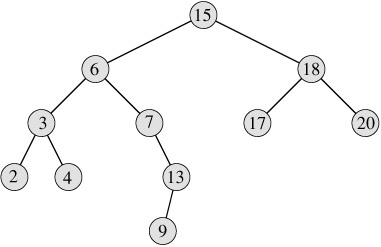
\includegraphics[scale=0.5]{img/tree.eps}
        \caption{example tree} \label{fig:example-tree}
       \end{center}
\end{figure}

\subsubsection*{C++ in-order walk testing and it's result.}

Suppose we have a pointer point to the tree contains data in figure 
\ref{fig:example-tree}. It can be created by build\_tree() function.

\lstset{language=C++}
\begin{lstlisting}
  struct Print{
    template<class T>
    void operator()(T x){ std::cout<<x<<", "; }
  };

  //...
  std::cout<<"test in order walk with print functor: ";
  in_order_walk(tree, Print());
\end{lstlisting}

In the above example, I created a function object Print, and pass an
instance of it to in-order walk process, it will print all the node
from less to greater with ',' as deliminator.

\begin{verbatim}
test in order walk with print functor: 2, 3, 4, 6, 7, 9, 13, 15, 
17, 18, 20,
\end{verbatim}

If boost::lambda is used, the above test cases can be simplied
a lot.
\begin{lstlisting}
//#include <boost/lambda/lambda.hpp> at the begin
using namespace boost::lambda;
std::cout<<"test in order walk with print functor: ";
in_order_walk(tree, std::cout<<_1<<", ");
\end{lstlisting}

While the Haskell version can be tested as below:

\lstset{language=Haskell}
\begin{lstlisting}
testTreeWalk = "test tree in-order walk by apply (-):\t"++
               show (inOrderWalk t2 (\x -> -x))

main = do
  putStrLn testTreeWalk
\end{lstlisting}

This test example 'maps' each keys in the tree to its negative value,
so it can output a result as below:

\begin{verbatim}
test tree in-order walk by apply (-):   Node (Node (Node 
(Node Empty (-2) Empty) (-3) (Node Empty (-4) Empty)) (-6) 
(Node Empty (-7) (Node (Node Empty (-9) Empty) (-13) 
Empty))) (-15) (Node (Node Empty (-17) Empty) (-18) (Node 
Empty (-20) Empty))
\end{verbatim}

% ================================================================
% Querying a binary search tree
% ================================================================
\section{Querying a binary search tree}

This section provides implementation of querying operations which are
described in 12.2 of CLRS\cite{CLRS}

\subsection{Searching}
In CLRS\cite{CLRS}, searching is demonstrated in both recursive way and 
imperactive way. According to the definition of binary search tree, search
a value in a tree can be realized in the following recursive manner.

\begin{itemize}
\item If the tree is empty, just return empty (not-found);
\item If the key of the root is equal to the value to be found, 
return the root;
\item If the value is less than the key of the root, search in the left
child.
\item Else, which means that the value is greater than the key of the 
root, search in the right child.
\end{itemize}

\subsubsection*{Haskell search implementation, recursive}
\lstset{language=Haskell}
\begin{lstlisting}
search::(Ord a)=> Tree a -> a -> Tree a
search Empty _ = Empty
search t x | key(t)==x = t
           | x < key(t) = search (left t) x
           | otherwise = search (right t) x
\end{lstlisting}

Hakell program of search is just translate the above recursive algorithm
description into code. Since it uses less than operator '<', the type
of the key value must be comparable. So the type variable is an instance 
of Ord type class.

\subsubsection*{C++ search implementation, imperactive}
\lstset{language=C++}
\begin{lstlisting}
template<class T>
node<T>* search(node<T>* t, T x){
  while(t && t->value!=x){
    if(x < t->value) t=t->left;
    else t=t->right;
  }
  return t;
}
\end{lstlisting}

Search can also be implemented in an imperactive way by replace the current
node to left child if the value to be search less than the key or to right 
child if greater than.

To test search programs, for C++, I defined a special version of assert, named
as assert\_(), it can write logs to stdout to tell if the test case ok or fail.

here is C++ version of search testing.

\lstset{language=c++}
\begin{lstlisting}
template<class T> void assert_(std::string msg, T x, T y){
  std::cout<<msg;
  if(x==y)
    std::cout<<x<<" OK.\n";
  else
    std::cout<<x<<"!="<<y<<" Fail.\n";
}

node<int>* empty(0);
assert_("search empty: ", search(empty, 3), empty);
std::cout<<"search exist value: "
         <<tree_to_str(search(tree, 18))<<"\n";
assert_("search non-exist: ", search(tree, 5), empty);
\end{lstlisting}

The variable tree is created as describe in above section. This test example 
gives the result as.
\begin{verbatim}
search empty: 0 OK.
search exist value: ((empty), 17, (empty)), 18, ((empty), 20, (empty))
search non-exist: 0 OK.
\end{verbatim}

Next is Haskell version of search testing.

\lstset{language=Haskell}
\begin{lstlisting}
testSearch = "\ntest search empty tree:\t"++ show (search 
                     (Empty::Tree Int) 3) ++
             "\ntest search non exist node in tree:\t"++ 
                     show (search t2 5)++
             "\ntest search a node in tree:\t"++ show 
                     (search t2 18)

main = do
  putStrLn testSearch
\end{lstlisting}

Where t2 is defined as the example tree, the result is:
\begin{verbatim}
test search empty tree: Empty
test search non exist node in tree:     Empty
test search a node in tree:     Node (Node Empty 17 Empty) 
18 (Node Empty 20 Empty)
\end{verbatim}


\subsection{Minimun and maximum}

Minimum and maximum can be implemented from the property of binary search
tree, less keys are always in left child, and greater keys are in right.

For minimum, we can continue traverse the left sub tree until it is empty.
While for maximum, we traverse the right.

\subsubsection*{C++ version of max/min, imperactive}

\lstset{language=c++}
\begin{lstlisting}
template<class T>
node<T>* min(node<T>* x){
  while(x && x->left)
    x = x->left;
  return x;
}

template<class T>
node<T>* max(node<T>* x){
  while(x && x->right)
    x = x->right;
  return x;
}
\end{lstlisting}

While in Haskell, in order not to conflict with the max/min functions 
defined in prelude, I change the name to maxt/mint.

\subsubsection*{Haskell version of max/min, recursive}
\lstset{language=Haskell}
\begin{lstlisting}
mint::Tree a -> Tree a
mint t = if isEmpty (left t) then t else mint (left t)

maxt::Tree a -> Tree a
maxt t = if isEmpty (right t) then t else maxt (right t)
\end{lstlisting}

\subsubsection*{test case and result in C++}
\lstset{language=c++}
\begin{lstlisting}
node<int>* empty(0);
assert_("min(empty)=", min(empty), empty);
assert_("min(tree)=", min(tree)->value, 2);
assert_("max(empty)=",max(empty), empty);
assert_("max(tree)=", max(tree)->value, 20);
\end{lstlisting}

\begin{verbatim}
min(tree)=2 OK.
max(empty)=0 OK.
max(tree)=20 OK.
search empty: 0 OK.
\end{verbatim}

\subsubsection*{test case and result in Haskell}

\lstset{language=Haskell}
\begin{lstlisting}
testMinMax = "\ntest min empty:\t" ++ 
               (show (mint (Empty::Tree Int))) ++
             "\ntest min tree:\t" ++ show (mint t2) ++ 
             "\ntest max empty:\t" ++ 
               (show (maxt (Empty::Tree Int))) ++
             "\ntest max tree:\t" ++ show (maxt t2)

main = do
    putStrLn testMinMax
\end{lstlisting}

\begin{verbatim}
test min empty: Empty
test min tree:  Node Empty 2 Empty
test max empty: Empty
test max tree:  Node Empty 20 Empty
\end{verbatim}

\subsection{Successor and predecessor}

Successor and predecessor is useful when a tree is treated as a generic container,
and traversed by using iterator. It will be relative easier to implement if parent of
a node can be accessed directly. The C++ version and python version benifit from
this reason.

\subsubsection*{C++ version of succ/pred, imperactive}

\lstset{language=C++}
\begin{lstlisting}
template<class T>
node<T>* succ(node<T>* x){
  if(x){
    if(x->right) return min(x->right);
    //find an ancestor, whose left child contains x
    node<T>* p = x->parent;
    while(p && p->right==x){
      x = p;
      p = p->parent;
    }
    return p;
  }
  return 0;
}

template<class T>
node<T>* pred(node<T>* x){
  if(x){
    if(x->left) return max(x->left);
    //find an ancestor, whose right child contains x
    node<T>* p = x->parent;
    while(p && p->left==x){
      x = p;
      p = p->parent;
    }
    return p;
  }
  return 0;
}
\end{lstlisting}

In function succ(), it takes a node in a tree, and tries to find the successor
of this node. if the node to be found is empty, it just returns it.

If the node has non-empty right child, the answer will be the min node in right
sub tree. While if it hasn't right sub tree, we must back track the ancestors 
of this node, try to find one, whose key is bigger. This can be approached 
by testing if the left child of an ancestor contains our node.

We can test the above program as below:

\begin{lstlisting}
assert_("succ 7: ", succ(search(tree, 7))->value, 9);
assert_("succ 13: ", succ(search(tree, 13))->value, 15);
assert_("succ 20: ", succ(search(tree, 20)), empty);
assert_("pred 6: ", pred(search(tree, 6))->value, 4);
assert_("pred 7: ", pred(search(tree, 7))->value, 6);
assert_("pred 2: ", pred(search(tree, 2)), empty);
\end{lstlisting}

And the result is:
\begin{verbatim}
succ 7: 9 OK.
succ 13: 15 OK.
succ 20: 0 OK.
pred 6: 4 OK.
pred 7: 6 OK.
pred 2: 0 OK.
\end{verbatim}

\subsubsection*{Haskell version of succ/pred, recursive}

In Haskell implementation, since I don't record parent for a node, it's hard
to find successor and predecessor in a easy way. I am not able to find a high
efficient way to realize them.

I defined some helper functions to find parent of a node in the tree, and filter
out the ancestor of a node which satisfies a predication. 

\lstset{language=Haskell}
\begin{lstlisting}
-- Find parent of a value in tree
-- The performance is low: O(h)
parent::(Ord a)=>Tree a -> a -> Tree a
parent Empty _ = Empty
parent t x | x < (key t) = if isParent (left t) x then t 
                              else parent (left t) x
           | x > (key t) = if isParent (right t) x then t 
                              else parent (right t) x
           | otherwise = Empty where
               isParent Empty _ = False
               isParent t x = (key t)==x

-- Find an ancestor of a value wich match a certain rule
-- Performance is very low.
findAncestor::(Ord a)=>Tree a -> a ->(a->a->Bool)-> Tree a
findAncestor t x f = checkParent t (parent t x) x f where
    checkParent _ Empty _ _ = Empty
    checkParent t p x f = if f (key p) x then p
                          else checkParent t (parent t (key p)) x f
\end{lstlisting}

The helper function, parent, takes 2 parameters, one is a tree, the other
is a value x. If the tree is empty, there is no parent, so the program returns
empty. In other case, it will test from root recursively to check if x is equal to
the key of the left sub tree root or right sub tree root.

The other helper function, findAncestor will utilize parent function. it takes 3
parameters, a tree, a value x, and a predicate function. the program will first 
check the direct parent of x matches the predicate. If succeeds, the parent will
be returned, else it will recursively check grand parent until finally reach to root.

With these 2 helpers, succ/pred can be realized as the following:
\begin{lstlisting}
-- Performance is very low.
succt::(Ord a)=>Tree a -> a -> Tree a
succt Empty _ = Empty
succt t x = if not (isEmpty rightNode)
            then mint rightNode
            else findAncestor t x (>) where
                rightNode = right (search t x)

-- Performance is very low
predt::(Ord a)=>Tree a -> a -> Tree a
predt Empty _ = Empty
predt t x = if not (isEmpty leftNode)
            then maxt leftNode
            else findAncestor t x (<) where
                leftNode = left (search t x)
\end{lstlisting}

For either cases, the program will fist call search function to locate the node
which key value is equal to x. In order to find the successor of a node, we'll 
check if the node has right child. If the right child isn't empty, the minimum 
of right sub tree is the answer, else we'll track back to find the nearest 
ancestor which is greater than x.

The test cases and result are as below:
\begin{lstlisting}
testSuccPred = 
  "\ntest succ of 7:\t"++ show (key (succt t2 7)) ++
  "\ntest succ of 13:\t"++ show (key (succt t2 13)) ++
  "\ntest pred of 6:\t"++ show (key (predt t2 6))++
  "\ntest pred of 7:\t"++ show (key (predt t2 7))

main = do
    putStrLn testSuccPred
    putStrLn testDel
\end{lstlisting}

\begin{verbatim}
test succ of 7: 9
test succ of 13:        15
test pred of 6: 4
test pred of 7: 6
\end{verbatim}

Note that there is a big problem in compute time of successor and predecessor 
operations if I implement them as above. For the imperactive version, the time
is $O(h)$, where $h$ is the height of the tree ($h$ close to $log(N)$ if the
binary search tree is balanced), while it is quite slow than this because each
parent/ancestor finding operation takes $O(h)$ time. I am finding if there is 
better solution.

% ================================================================
%                 Insertion and deletion
% ================================================================
\section{Insertion and deletion}

Different with all above tree operations, insertion and deletion can mutate
the tree. All functions I defined till now are 'read only' functions.

\subsection{Insertion}
Insertion is the neccessary element to create a tree, one recursive description
of insertion is like this.

To insert a value x to a tree t,
\begin{itemize}
\item If the tree is empty, then return a leave with key=x;
\item If x is less than the key of root node, insert x to the left child;
\item If x is greater than the key of root, insert x to the right child.
\end{itemize}

\subsubsection*{Haskell tree insertion, recursive}
By translate the above description into Hasell code, the program can be written
as below.

\begin{lstlisting}
insert::(Ord a) => Tree a -> a -> Tree a
insert Empty x = leaf x
insert t x = if x < key(t) 
             then (Node (insert (left t) x) (key t) (right t))
             else (Node (left t) (key t) (insert (right t) x))
\end{lstlisting}

The testing of insertion can be found in section \ref{list2tree}

\subsubsection*{C++ tree insertion, imperactive}

By using imperacitve language such as C++, we can iterate to the sub-tree untill
to the insertion point. There are some extra lines to set the parent of the node
properly.

\lstset{language=C++}
\begin{lstlisting}
template<class T>
node<T>* insert(node<T>* tree, T value){
  node<T>* root(tree);
  node<T>* x = new node<T>(value);
  node<T>* parent(0);
  while(tree){
    parent = tree;
    if(value < tree->value)
      tree = tree -> left;
    else //assert there is no duplicated value inserted.
      tree = tree -> right;
  }
  x->parent = parent;
  if( parent == 0 ) //tree is empty
    return x;
  else if( value < parent->value)
    parent->left = x;
  else
    parent->right = x;
  return root;
}
\end{lstlisting}

The testing can be refer to section \ref{list2tree}.

\subsection{Deletion}
Deletion is the most complex operation for binary search tree. this is because we
must keep the property, that left sub tree < key < right sub tree. Deleting a node
can break this property very easy.

I don't use the same algorithm described in CLRS\cite{CLRS}, I found a more simple
one from 'Annotated STL'\cite{hj-stl}

The algorithm can be described as below:

To delete a node x from a tree.
\begin{itemize}
\item If x has no child or only one child, splice x out;
\item If x has two children, use minimun of its right to replace x, 
and splice the original minimum out.
\end{itemize}

\subsubsection*{Haskell deletion, recursive}

Haskell version of deletion can be realized by translating the above descrition
directly into code. But there is a different point, instead of pass a node to the
function, I pass value to be deleted in it. So the program need perform search first.

\lstset{language=Haskell}
\begin{lstlisting}
delete::(Ord a)=> Tree a -> a -> Tree a
delete Empty _ = Empty
delete (Node l k r) x | x < k = (Node (delete l x) k r)
                      | x > k = (Node l k (delete r x))
                      -- x == k
                      | isEmpty l = r
                      | isEmpty r = l
                      | otherwise = (Node l k' (delete r k')) 
                          where k' = key (mint r)
\end{lstlisting}

The test cases and result are shows as below.

\begin{lstlisting}
testDel = "\ntest del 17:\t"++ show (delete t2 17)++
          "\ntest del 7:\t"++ show (delete t2 7)++
          "\ntest del 6:\t" ++ show (delete t2 6)++
          "\ntest del 15:\t"++ show (delete t2 15)++
          "\ntest del non-exist:\t" ++ show (delete t2 5)

main = do
    putStrLn testDel
\end{lstlisting}

\begin{verbatim}
test del 17:    Node (Node (Node (Node Empty 2 Empty) 3 (Node Empty 4 
Empty)) 6 (Node Empty 7 (Node (Node Empty 9 Empty) 13 Empty))) 15 
(Node Empty 18 (Node Empty 20 Empty))
test del 7:     Node (Node (Node (Node Empty 2 Empty) 3 (Node Empty 4 
Empty)) 6 (Node (Node Empty 9 Empty) 13 Empty)) 15 (Node (Node Empty 
17 Empty) 18 (Node Empty 20 Empty))
test del 6:     Node (Node (Node (Node Empty 2 Empty) 3 (Node Empty 4 
Empty)) 7 (Node (Node Empty 9 Empty) 13 Empty)) 15 (Node (Node Empty 
17 Empty) 18 (Node Empty 20 Empty))
test del 15:    Node (Node (Node (Node Empty 2 Empty) 3 (Node Empty 4 
Empty)) 6 (Node Empty 7 (Node (Node Empty 9 Empty) 13 Empty))) 17 
(Node Empty 18 (Node Empty 20 Empty))
test del non-exist:     Node (Node (Node (Node Empty 2 Empty) 3 (Node 
Empty 4 Empty)) 6 (Node Empty 7 (Node (Node Empty 9 Empty) 13 Empty))) 
15 (Node (Node Empty 17 Empty) 18 (Node Empty 20 Empty))
\end{verbatim}

\subsubsection*{C++ deletion, imperactive}

C++ version is more complex because it need set the parent properly.
While we can pass the pointer to the node which will be deleted to the function,
so that search is no more needed. The function will return the root
of the result tree.

\lstset{language=C++}
\begin{lstlisting}
template<class T>
node<T>* del(node<T>* tree, node<T>* x){
  if(!x)
    return tree;

  node<T>* root(tree);
  node<T>* old_x(x);
  node<T>* parent(x->parent);

  if(x->left == 0)
    x = x->right;
  else if(x->right == 0)
    x = x->left;
  else{
    node<T>* y=min(x->right);
    x->value = y->value;
    if(y->parent != x)
      y->parent->left = y->right;
    else
      x->right = y->right;

    remove_node(y);
    return root;
  }

  if(x)
    x->parent = parent;

  if(!parent)
    root = x; //remove node of a tree
  else
    if(parent->left == old_x)
      parent->left = x;
    else
      parent->right = x;

  remove_node(old_x);
  return root;
}
\end{lstlisting}

If the node to be deleted is empty, the function simply returns the original tree.
In other cases, it will first record the root of the tree, create a copy pointer
to x, and to its parent.

If either of the children is empty, the program just splice x out. If it has two
none-empty children, we first located the minimun of right child, replace the key
of x to y's, then splice y out. Note that the helper function remove\_node() is
used.

Finally we reset the parent. If the parent pointer we copied before is empty, it
means that we are deleting the root node, so we need return the new root. After
the parent is set properly, we finally remove the old x from memory.

The test cases and result are shows as below.

\begin{lstlisting}
void test_del_n(int n){
  node<int>* empty(0);
  node<int>* t1=clone_tree(tree);
  t1=del(t1, search(t1, n));
  std::cout<<"del "<<n<<":\n"<<tree_to_str(t1)<<"\n";
  assert_("search after del: ", search(t1, n), empty);
  delete t1;
}

test_del_n(17);
test_del_n(7);
test_del_n(6);
test_del_n(15);
test_del_n(1); //try to del a non-exist val
\end{lstlisting}

Because the deletion function in C++ inplace change the tree, so I cloned the test 
tree for each testing. The clone\_tree() function is defined in section \ref{helper-fun}.

The result of these test case is as below.
\begin{verbatim}
del 17:
((((empty), 2, (empty)), 3, ((empty), 4, (empty))), 6, ((empty), 7, 
(((empty), 9, (empty)), 13, (empty)))), 15, ((empty), 18, ((empty), 
20, (empty)))
search after del: 0 OK.
del 7:
((((empty), 2, (empty)), 3, ((empty), 4, (empty))), 6, (((empty), 9, 
(empty)), 13, (empty))), 15, (((empty), 17, (empty)), 18, ((empty), 
20, (empty)))
search after del: 0 OK.
del 6:
((((empty), 2, (empty)), 3, ((empty), 4, (empty))), 7, (((empty), 9, 
(empty)), 13, (empty))), 15, (((empty), 17, (empty)), 18, ((empty), 
20, (empty)))
search after del: 0 OK.
del 15:
((((empty), 2, (empty)), 3, ((empty), 4, (empty))), 6, ((empty), 7, 
(((empty), 9, (empty)), 13, (empty)))), 17, ((empty), 18, ((empty), 
20, (empty)))
search after del: 0 OK.
del 1:
((((empty), 2, (empty)), 3, ((empty), 4, (empty))), 6, ((empty), 7, 
(((empty), 9, (empty)), 13, (empty)))), 15, (((empty), 17, (empty)), 
18, ((empty), 20, (empty)))
search after del: 0 OK.
\end{verbatim}

\section{Appendix} \label{appendix}
%\appendix
All programs are provided along with this article. They are free for downloading.
\begin{itemize}
\item bstree.cpp, C++ version of binary seach tree, including all test cases. I 
compiled and tested it with GUN G++ 3.4.4.
\item BSTree.hs, Haskell version of binary search tree, with test cases. I compiled
and tested it with GHC 6.10.4.
\end{itemize}
download position: http://sites.google.com/site/algoxy/bstree/bstree.zip

\begin{thebibliography}{99}

\bibitem{CLRS}
Thomas H. Cormen, Charles E. Leiserson, Ronald L. Rivest and Clifford Stein. 
``Introduction to Algorithms, Second Edition''. ISBN:0262032937. The MIT Press. 2001

\bibitem{hj-stl}
Hou Jie. ``The annotated STL sources (using SGI STL)''. ISBN:7-5609-2699-1 http://press.hust.edu.cn. 2002.

\bibitem{literal-program}
http://en.literateprograms.org/Binary\_search\_tree\_(Haskell)

\end{thebibliography}

\ifx\wholebook\relax\else
\end{document}
\fi
